\documentclass[12pt, a4paper]{article}

\usepackage[utf8]{inputenc}
\usepackage[ngerman]{babel}
\usepackage{amsmath, amssymb}
\usepackage[left=2.5cm, right=2.5cm, top=2.5cm, bottom=2.5cm]{geometry}
\usepackage{graphicx}
\usepackage{fancyhdr}
\usepackage{titling}
\usepackage{caption}
\usepackage{subcaption}
\usepackage{setspace}
\usepackage{footmisc}
\usepackage[colorlinks=false, pdfborder={0 0 0}]{hyperref}
\usepackage[font=footnotesize,labelfont=bf]{caption}
\usepackage[format=plain, indention=2em]{caption}
\graphicspath{{Image Sources/}}

\newcommand{\subtitle}[1]{%
	\posttitle{%
		\par\end{center}
	\begin{center}\large#1\end{center}
	\vskip0.5em}%
	}
	
\addto\captionsngerman{\renewcommand{\figurename}{Fig.}}
\onehalfspacing
\renewcommand{\subsectionmark}[1]{}
\renewcommand{\footnotelayout}{\setstretch{1.0}\footnotesize}
\renewcommand{\labelenumi}{\Roman{enumi}}
\renewcommand{\labelenumii}{\Roman{enumi}.\roman{enumii}}
\renewcommand{\labelenumiii}{\Roman{enumi}.\roman{enumii}.\roman{enumiii}}
\renewcommand{\labelenumiv}{\Roman{enumi}.\roman{enumii}.\roman{enumiii}.\roman{enumiv}}



\title{W-Seminar}
\subtitle{Deckblatt siehe ByCs}
\author{Armin Binder }
\date{SJ 2024/25}

\begin{document}
	\pagestyle{fancy}
	\fancyhf{} 
	\fancyfoot[C]{\thepage}
	
	%\pagenumbering{arabic}
%	\fancyhf{}
%	\fancyfoot[R]{\thepage}
	\maketitle
	\thispagestyle{empty}
	\pagebreak
	
	\tableofcontents
	\thispagestyle{empty}
	\pagebreak
	
	\section{Abstract}
	
	
	\section{Einleitung}
	\subsection{Geschichte und Bedeutung von Magnetfeldern und ihrer Messung - Obsolet}
		
	\subsection{Magnetfeldmessungen und der Hall-Effekt - Überarbeiten; Beschreibungen Methoden in Anhang}
	
	Über diese lange Geschichte der Magnetfeldforschung wurden auch dementsprechend viele verschiedene Methoden entwickelt um Magnetfelder zu messen, die von sehr einfachen Methoden bis hin zu hochkomplexen Quantenmethoden reichen. Hier eine kurze Zusammenfassung einiger relevanter Messmethoden:
	\begin{itemize}
		\item \textbf{Magnetresonanzmessungen:} Wasser, entweder als kleine Probe oder fließend durch eine kleine Röhre, wird in einer Anregungsspule von Radiowellen angeregt. Das magnetische Moment der Wassernukleonen, beeinflusst durch ein externes Magnetfeld, wird entweder über nukleare Induktion\footnote{Induktionseffekte, die durch das magnetische Moment von Nukleonen hervorgerufen werden} oder über Resonanzabsorption ausgelesen
		\item \textbf{Magnetische Flussmeter:} Durch Änderungen des Magnetfelds wird in einer Messspule eine Spannung induziert. Diese Spannung wird über die Zeit integriert, um den magnetischen Fluss zu bestimmen
		\item \textbf{Photoelektrische Flussmeter:} Durch ein Magnetfeld wird eine Bewegung erzeugt, die in ein Lichtsignal umgewandelt und von einem Photosensor gemessen wird, um den magnetischen Fluss zu bestimmen
		\item \textbf{Hall-Methode:} An einen kleinen Metall- oder Halbleiterstreifen wird eine Anregungsspannung angelegt. Wirkt ein Magnetfeld auf die bewegten Ladungsträger, werden diese durch die Lorentzkraft seitlich abgelenkt. Dadurch entsteht eine messbare Hall-Spannung quer zum Stromfluss, aus der die Stärke des Magnetfelds bestimmt werden kann
		\item \textbf{Fluxgate-Magnetometer:} Um einen ferromagnetischen Kern werden mindestens drei Spulen angebracht:
			\subitem - Eine Wechselstrom-Anregungsspule, die den Kern  alternierend sättigt 
			\subitem - Eine Messspule, an der im Idealfall immer eine Nullspannung anliegt
			\subitem - Eine Gleichstrom-Bias-Spule, die ein externes Magnetfeld ausgleicht, sodass die Messspule wieder Nullspannung ausliest
			\newline
		Aus der Höhe des Gleichstroms, der zur Neutralisierung des Feldes benötigt wird, lässt sich die Stärke des externen Magnetfelds bestimmen
		\item \textbf{Magneto-Resistenz-Messungen:}
		\item \textbf{Visuelle Magnetfeldkartierung:}
		\item \textbf{Teilchenstrahl-Beobachtung: }
		\item \textbf{Atomare Magnetometer:}
		\item \textbf{Spin-Exchange-Relaxationsfreies (SERF) Magnetometer:}
		\item \textbf{Optisch gepumptes Magnetometer (OPM):}
		\item \textbf{Supraleitende Quanteninterferenzgeräte:}
	\end{itemize}
	
	
	\subsection{Projektziel und thematischer Bezug}
	
	
	\section{Funktionsweise der X-Hall-Architektur}
		Im vorherigen Kapitel wurden bereits die grundlegende Funktionsweise von Hall-Sensoren sowie typische Architekturen solcher Systeme behandelt.\paragraph{}
		Die für diese Arbeit gewählte Architektur, die sogenannte \textbf{X-Hall-Architektur} unterscheidet sich jedoch von den zuvor genannten Architekturen in mehreren relevanten Aspekten. Im Folgenden soll diese spezifische Architektur vorgestellt werden und auf ihre Vor- sowie Nachteile eingegangen werden, ebenso wie auf die Gründe zur Wahl genau dieser %genauen 
		Architektur für diese Arbeit.
		
		\subsection{Geschichte und Konzept}
		Bei der X-Hall-Architektur handelt es sich um eine recht neue Form des Hall-Sensors. Erstmalig wurde sie gegen Ende des Jahres 2018 auf dem IMEKO\footnote{International Measurement Confederation} 
		World Congress vorgestellt \textbf{\cite{cres19}}. \newline
		Die Entwicklung dieser neuen Art Hall-Sensor wurde insbesondere durch den Bedarf für Magnetfeldsensoren mit immer größeren Frequenzbandbreiten vorangetrieben, die grundlegende Bestandteile unter anderem von Sicherheitsschaltungen vieler moderner Stromversorgungskreisläufe sind\textbf{\cite{cres18}\cite{cres19}\cite{cres20}\cite{cres21}}. Die bisher genutzten Sensortypen und Architekturen, wohlgemerkt nicht exklusiv Hall-Sensoren, wiesen aber bereits durch ihren Aufbau alle gewisse Einschränkungen und Probleme auf, die ihre Einsetzbarkeit limitierten\textbf{\cite{cres18}\cite{cres19}\cite{cres21}}. \newline
		Ziel der neuen Sensorarchitektur sollte es also sein, alle Aspekte, die für so einen Magnetfeldsensor relevant sind, in sich zu vereinen\textbf{\cite{cres19}}: 
		\begin{itemize}
			\item Sehr hohe bemessbare Frequenzbandbreiten von Magnetfeldern %Nochmal seperat bestätigen
			\item Fähigkeiten, Gleichspannung (indirekt) zu messen
			\item Mögliche CMOS\footnote{Complementary Metal-Oxide Semiconductor = komplementärer Metalloxid-Halbleiter}-Integration
			\item Galvanische Isolation\footnote{Elektrische funktionale Sektionen sind so voneinander isoliert, dass es keinen direkten Stromfluss zwischen ihnen gibt}
			\item Keine Wärmeabstrahlung
			\item Geringer Flächenbedarf %Kleines Profil
			\item Geringe Produktionskosten
		\end{itemize} 
		Aus diesen Überlegungen resultierte die Entwicklung der sogenannten X-Hall-Architektur\newline
		Einfach gesagt handelt es sich hierbei um eine Hall-Sonde mit jeweils vier Vorspannungs\footnote{Strom der durch den Sensor fließt, um den Hall-Effekt erst zu ermöglichen}- und vier Auslesekontakten (was jeweils das doppelte der jeweiligen Kontaktarten bei typischen Hall-Sensoren ist), die an der aktiven Fläche des Sensors angebracht sind. Durch eine elektrische Verbindung jeweils zweier diagonal gegenüberliegender Auslesekontakte vor dem eigentlichen Auslesevorgang wird gewährleistet, dass mögliche Defekte und Offsetspannungen\footnote{Ungewollte Spannungen, die selbst dann gemessen werden können, wenn der theoretische Messwert 0 sein sollte} auf der größeren aktiven Fläche unter anderem durch so entstehende Mittelungseffekte kompensiert werden. Dies führt zu einer einer höheren Genauigkeit und Stabilität der Messwerte.
		
		\subsection{Aufbau und Funktionsweise}
		Bei der aktiven Fläche eines X-Hall-Sensors handelt es sich in der Regel um einen oktagonal geformten, sogenannten n-Well\footnote{n-dotierte ``Halbleitertasche'' innerhalb eines p-dotierten Substrats} \cite{cres18}. \newline
		Die n-Dotierung der aktiven Sensorfläche wird aufgrund einer höheren strombezogenen Empfindlichkeit\footnote{Begründet durch höhere Elektronenmobilität in n-Typ-Halbleitern} im Gegensatz zu p-dotierten Halbleitern präferiert. %bevorzugt?
		Auch ist die Umschließung des n-Wells mit einem p-dotierten Material zwar für die grundlegende Sensorfunktion nicht essenziell, %auf nichtverwendung in Arbeit aufgrund komplexität hinweisen? 
		sollte jedoch  angestrebt werden, da nur so eine effektive elektrische Isolation gegenüber dem Substrat erreicht werden kann\cite{cres20}.\newline
		Der Zugang zur aktiven Fläche erfolgt über insgesamt acht Kontakte, die sich in vier großflächige Vorspannungskontakte und vier möglichst kleine Auslesekontakte unterteilen lassen. Die Vorspannungskontakte profitieren aufgrund ihrer Größe von sehr niedrigen Widerständen beim Anlegen der Vorspannung, während die Auslesekontakte so klein wie möglich sein sollten, da so mögliche parasitäre Kapazitätseffekte\footnote{Unerwünschte Kapazität, die durch geringe physische Nähe zwischen elektrischen Bauteilen entsteht} % , ???
		wie Signalverzerrungen oder Rauschen minimiert werden können.\cite{cres19}.\newline
		An die in Fig.~\ref{fig:3}(a) als B und T bezeichneten Vorspannungskontakte werden nominal gleiche Vorspannungsströme ($I_A=I_B$) angelegt, während die als L und R bezeichneten Kontakte jeweils als Erdungskontakte dienen\cite{cres19}. Die Auslesekontakte sind von 1 bis 4 durchnummeriert.\newline
		In der aktuellen Konfiguration kann die gesamte Sensorsonde in zwei innere Sensorsonden untergliedert werden, die in Fig.~\ref{fig:3}(a) als Probe A und Probe B bezeichnet sind. Dies Aufteilung ergibt sich direkt aus der in Fig.~\ref{fig:3}(b) dargestellten Stromstärkeverteilung zwischen den Kontakten auf dem Halbleiter, da der Strom über die Erdung bereits abgeführt wird, bevor er die zweite innere Sonde erreichen kann\cite{cres20}.
		\begin{figure}
			\centering
				%Fig. 1-a
				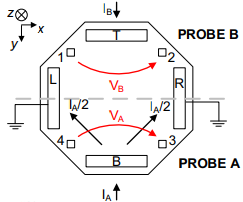
\includegraphics[height=5cm]{Fig3.1}	
				\hspace{0.5cm}
				%Fig. 1-b
				
\includegraphics[height=5cm]{Fig3.2}
				\caption{(a) Skizze des Aufbaus der X-Hall-Sonde, (b) Stromstärkeverteilung auf der X-Hall-Sonde, basierend auf einer beispielhaften Vorstromstärke von $I_A=I_B=500\mu{A}$}
				\label{fig:3}
		\end{figure}\newline
		Diese inneren Sonden funktionieren, unabhängig voneinander, jeweils wie gewöhnliche stromverzweigende Hall-Sonden, bei denen die jeweilige Stromdichte $J_A$ oder $J_B$ in zwei gleiche Stromdichten $J_{A,L}$ und $J_{A,R}$ beziehungsweise $J_{B,L}$ und $J_{B,R}$ aufgespalten werden. Dementsprechend gilt für jeweiligen Potentiale zwischen den Messkontakten 1 und 2 beziehungsweise 3 und 4 in Abwesenheit eines Magnetfelds: $V_A=V_B=0$ \cite{cres21}.\newline
		Liegt nun ein Magnetfeld $B_Z$ vor, entsteht aufgrund der Lorentzkräfte die auf die Ladungsträger wirken ein Ungleichgewicht im Stromfluss, was dazu führt, dass nun vereinfacht $V_A=V_\mathrm{Hall}$ und $V_B=-V_\mathrm{Hall}$ (Da der Stromfluss in der zweiten inneren Sonde in die entgegengesetzte Richtung des Stroms von Sonde A verläuft).\newline
		In Realität lassen sich jedoch Asymmetrien in der Sensorstruktur, globale Inhomogenitäten von Materialien und andere Defekte nicht vermeiden, weshalb für die gemessenen Spannungen $V_A$ und $V_B$ tatsächlich gilt:
		\begin{equation}
			V_A=V_\mathrm{H,Sonde}+V_\mathrm{OS}^{(A)}
			\label{eq:1}
		\end{equation}
		\begin{equation}
			V_B=-V_\mathrm{H,Sonde}+V_\mathrm{OS}^{(B)}
			\label{eq:2}
		\end{equation}
		$V_\mathrm{OS}^{(A)}$ und $V_\mathrm{OS}^{(B)}$ sind die Offsetspannungen der jeweiligen inneren Sonde\cite{cres20}.\newline
		Da beide inneren Sonden sich nichtsdestotrotz die gleiche aktive Sensorfläche teilen, kann angenommen werden, dass das Vorzeichen von $V_\mathrm{OS}^{(A)}$ und $V_\mathrm{OS}^{(B)}$ identisch ist, auch wenn sich ihre jeweiligen Werte aufgrund lokaler Defekte unterscheiden können\cite{cres21}. Deshalb kann angenommen werden, dass die Hauptquelle der Offsets sehr wahrscheinlich für beide inneren Sonden die selbe ist\cite{cres20}.\newline
		\begin{figure}
			\centering
			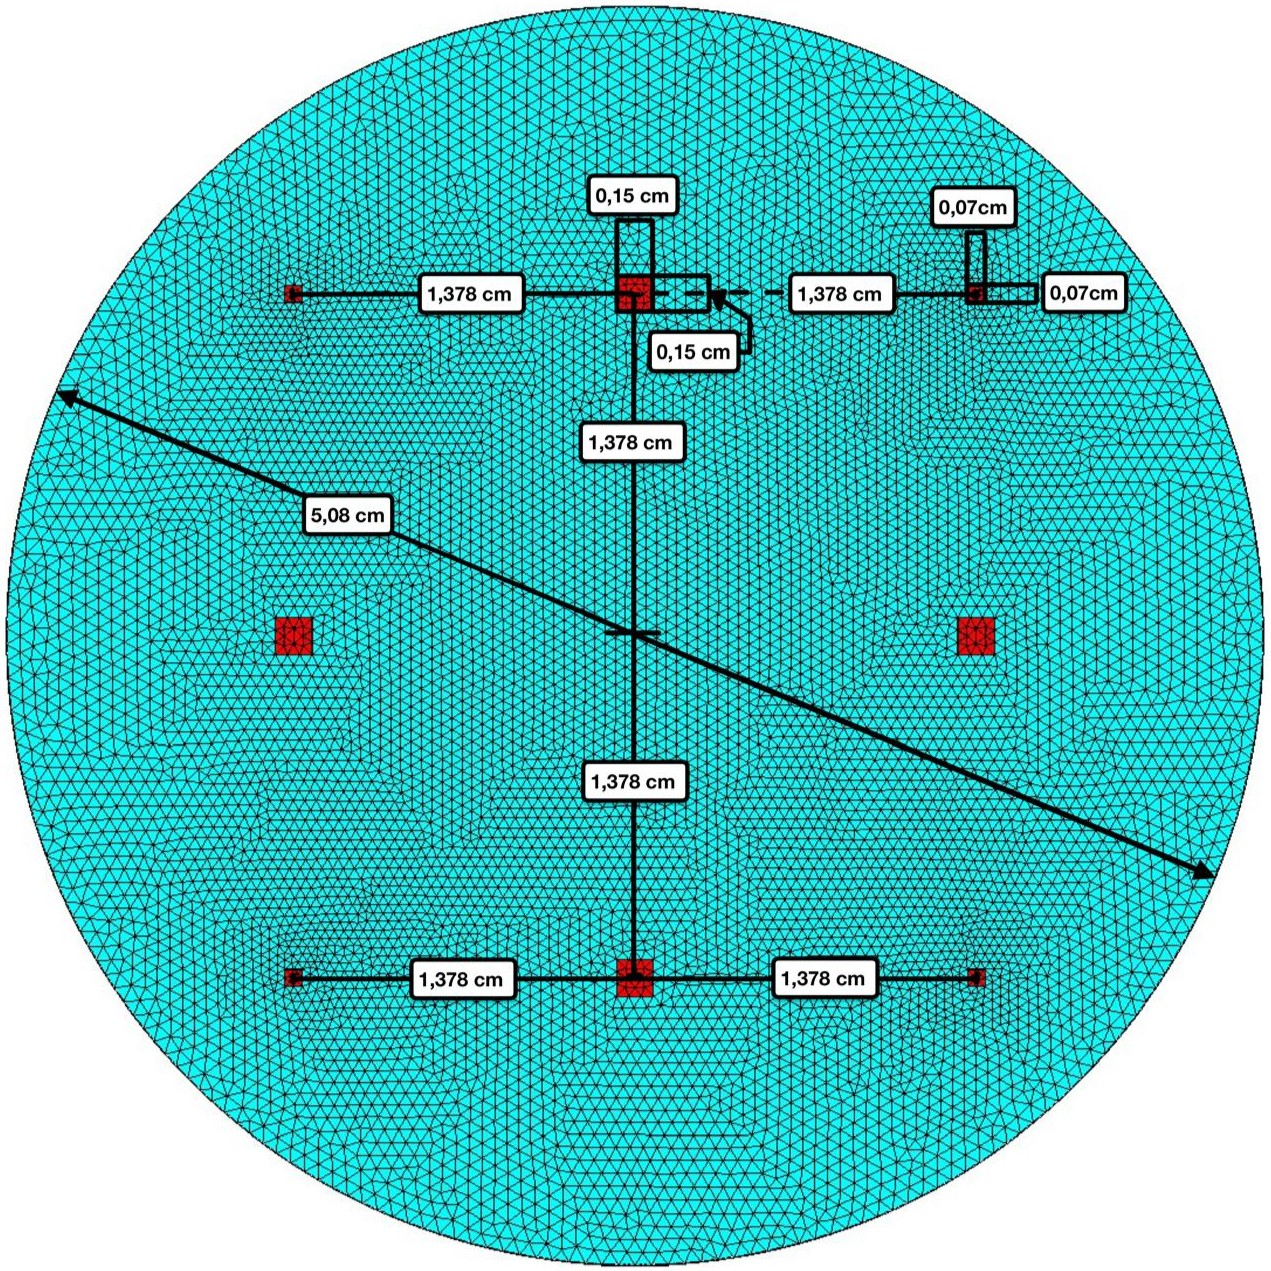
\includegraphics[height=5cm]{Fig4}
			\caption{Schematischer Schaltplan einer X-Hall-Sonde}
			\label{fig:4}
		\end{figure}
		Wie in Fig.~\ref{fig:4} gezeigt besteht die eigentliche und namensgebende Besonderheit der X-Hall-Architektur in einer Überkreuzverbindung der diagonal gegenüberliegenden Paare von Auslesekontakte (1 mit 3 und 2 mit 4). Daraus folgt:
		\begin{equation}
			V_A=-V_B=V_\mathrm{H,Sonde}
			\label{eq:3}
		\end{equation}
		Unter der Annahme gleicher Vorzeichen beider Offsetspannungen und einer Substitution von (\ref{eq:1}) und (\ref{eq:2}) in (\ref{eq:3}) wird  impliziert:
		\begin{equation}
			V_\mathrm{OS}^{(A)}=V_\mathrm{OS}^{(B)}=0
			\label{eq:4}
		\end{equation}
		Physikalisch gesehen erzeugt die Überkreuzverbindung der Auslesekontakte eine  Randbedingung in der aktiven Fläche, welche die Ladungsverteilung so beeinflusst, dass Offsetspannungen minimiert werden \cite{cres21}. 
		Durch die Überkreuzverbindung sind beide Kontakte elektrisch verbunden, was dazu führt, dass sich die Ströme der beiden Kontakte gegenseitig ausbalancieren. %Dies ist Teil der typischen Ladungsverteilung hin zum energetisch günstigsten Zustand des Systems. 
		Aufgrund dieser ladungsverschiebenden Effekte gleicht das System selbstständig ungewollte Offsets oder Defekte und damit verbundene energetisch ungünstige Ladungsverteilungen – ob lokal oder global – aus. %da das System bestrebt ist, seinen energetisch günstigen Zustand zu erreichen. 
		So werden Anteile dieser ungünstigen Ladungsverteilungen in den tatsächlich ausgelesenen Messwerten minimiert.\newline
		Trotzdem wird es immer vereinzelte lokale Defekte und Offsets geben, die zu einer verbleibenden Offsetspannung führen und jeweils zu $V_A$ und $V_B$ hinzugerechnet werden müssen. Die X-Hall-Architektur strebt also primär an, globale Defekte und Offsets mit starkem Einfluss auf Messergebnisse auszugleichen und nicht, diese vollständig zu eliminieren\cite{cres21}.
		
		\subsection{Vorteile und Nachteile der Architektur}
		Die eigentlichen Anforderungen an die X-Hall-Architektur wurden bereits in Kapitel 3.1 behandelt. Auf theoretischer Ebene sollte die Architektur diese auch alle erfüllen.\newline
		Praktisch zeigt sich folgendes Bild:\paragraph{}
		
		Nach \cite{cres21} hat die X-Hall-Architektur das Potential, bis zu 200\,MHz oder mehr Messbandbreite zu realisieren, ohne dabei wie zuvor bestehende Lösungen hochkomplex in der Umsetzung zu sein. In der Praxis wurden bisher jedoch maximal Sensorbandbreiten um  20\,MHz\cite{cres19} erreicht.\newline
		Dies lässt sich vor allem dadurch erklären, dass für höhere Bandbreiten keine Stabilität der Messwerte und der Messwertverstärkung mehr zu garantieren ist, insbesondere Aufgrund perturbativer, induzierter Effekte in Anschlusskabeln und parasitärer Effekte.\paragraph{}
		Des Weiteren wird eine frequenzunabhängige Offsetkompensation erreicht, wobei hochentwickelte Spinning-Current-Hall-Sensoren immer noch wesentlich geringere Offsets erreichen können, dafür aber wesentlich geringere Bandbreiten haben. In \cite{cres22} wird konkret von $\Delta{V_{OS}}=116\,\mu{V}\pm1\mu{V}$ für den dort verwendeten X-Hall-Sensor gesprochen, während Spinning-Current-Modelle bis $\Delta{V_{OS}}=15\,\mu{V}$ und niedriger reichen können. Anzumerken ist, dass die von X-Hall-Sensoren erreichten Offsets aber trotzdem verhältnismäßig gering sind, wenn man sie mit anderen Sensoren vergleicht.\paragraph{}
		\cite{cres22} und \cite{cres23} zeigen weiter auf, dass die X-Hall-Architektur verhältnismäßig "limitierte Sensitivität" im Vergleich zu anderen Sensorarchitekturen besitzt. So wird in \cite{cres21Hall} dem X-Hall-Sensor eine Sensitivität von 36\,mv/A zugeordnet, während fast alle anderen dort aufgeführten Hall-Sensoren höhere Sensitivität bis zu 100\,mv/A aufweisen (Hohe Sensibilität ist für Detektion von schwachen Feldern essenziell). 
		
		
		\subsection{(Erwartete) Leistungscharakteristika der Architektur}
		Aufgrund des noch jungen Entwicklungsstands ist die Architektur bislang kaum verbreitet. Dementsprechend lassen sich die zu erwartenden Leistungscharakteristika am zuverlässigsten aus den bislang realisierten Sensoren in STMicroelectronics BCD\footnote{Bipolar-CMOS-DMOS} 160\,nm Technologie ableiten.\paragraph{}
		
		Aus \cite{cres18} lässt sich herauslesen, dass für einen Hall-Sensor dieser Spezifikation die durchschnittliche $\Delta{V_{OS}}=-0.27\,mV$, wobei eine sehr hohe Standardabweichung von $\sigma=0.64\,mV$ vorliegt.\newline
		Bei längerer Betriebsdauer sind nach \cite{cres23} Standardabweichungen von etwa $\sigma=26\,mA$ und Offset-Drifts von etwa 0,33\,mA/h zu erwarten, was äquivalent zu Magnetfeldern mit einer Streuung von etwa $\sigma=197\,\mu{T}$ und einem Drift von etwa $2.5\,\mu{T}/h$ ist.\footnote{\cite{cres23} nutzt eine modifizierte Variante des Sensors, der statt einer Spannung eine Stromstärke ausgibt; \cite{cres21} bestätigt diese Werte aber in etwa}\newline
		Für die wahrscheinlichere Temperaturregion des Sensors von etwa 30\,°C bis 100\,°C ist ein Temperaturkoeffizient von etwa -4.1\,mA/°C laut \cite{cres23} zu erwarten.\newline
		Die Sensitivität liegt nach \cite{cres21Hall} bei etwa 36\,mV/A, die dynamische Reichweite bei 52\,dB\footnote{Verhältnis von etwa 1:398 vom kleinsten zum größten messbaren Magnetfeld} und das Rauschen bei unter 100\,mA RMS / 3.6\,mV RMS.\newline
		Wir nehmen eine Bandbreite des Sensors von etwa 4\,MHz an\cite{cres21}. \paragraph{}
		
		Aufgrund der hohen erreichbaren Sensorbandbreite, der frequenzunabhängigen Offsetkompensation und insbesondere der einfachen Architektur und Implementierung im Vergleich zu anderen geeigneten Sensordesigns eignet sich die X-Hall-Architektur besonders gut für experimentelle Eigenentwicklungen, wie sie im weiteren Verlauf dieser Arbeit umgesetzt wird. %/Aufgrund der hohen erreichbaren Bandbreite, der frequenzunabhängigen Offsetkompensation und der vergleichsweise einfachen Implementierung eignet sich die X-Hall-Architektur besonders gut für experimentelle Eigenentwicklungen wie die im Rahmen dieser Arbeit umgesetzte.
		
	\section{Praktische Umsetzung des X-Hall-Sensors}
	
	\subsection{Die Finite Element Methode}
	
	\subsection{Entwicklung eines Sensor-Layouts - Include reasoning for choice of x-hall}
	
	\subsection{Praktische Implementierung des Sensors}
		
		
	\section{Vergleich mit anderen Hall-Sensoren}
	\subsection{Quantitativer Vergleich}
	
	\subsection{Qualitativer Vergleich}	
		
	\section{Fazit}
		
		
		
		
		
	\section*{%Literaturverzeichnis%
		}	%\clearpage
	\newpage
	\begin{thebibliography}{}
		\addcontentsline{toc}{section}{Literaturverzeichnis}
		
		\bibitem{paun13}
		\textbf{Maria-Alexandra Paun, JM. Salesse, M. Kayal}, Hall Effect Sensors Design, Integration and Behavior Analysis. Journal of Sensors and Actuator Networks, 2013, 2, pp. 85-97, doi: 10.3390/jsan2010085
		
		\bibitem{cres18}
		\textbf{M. Crescenti et. al.}, Bandwith enhancement in Hall Probe by X-Hall DC biasing. XXII World Congress of International Measurement Confederation (IMEKO 2018), Journal of Physics: Conf. Series \textbf{1065} (2018) 052031, Belfast, United Kingdom, 2018, doi: 10.1088/1742-6596/1065/5/052031
		
		\bibitem{cres19}
		\textbf{M. Crescenti et. al.}, A  Broadband Current Sensor based on the X-Hall Architecture. 2019 26th IEEE International Congerence on Electronics, Circuits and Systems (ICECS), Genoa, Italy, 2019, pp. 807-810, doi: 10.1109/ICECS46596.2019.8964955
		
		\bibitem{cres20}
		\textbf{M. Crescenti et. al.}, Experimental Assessment of a Broadband Current Sensor based on the X-Hall Architecture. 2020 IEEE International Instrumentation and Measurement Technology Conference (I2MTC), Dubrovnik, Croatia, 2020, pp. 1-6, doi: 10.1109/I2MTC43012.2020.9128994
					
		\bibitem{cres21}
		\textbf{M. Crescenti et. al.}, The X-Hall Sensor: Towards Integrated Broadband Current Sensing. IEEE TRANSACTIONS ON INSTRUMENTATION AND MEASUREMENT, vol. 70, pp. 1-12, 2021, doi: 10.1109/TIM.2020.3036764
		
		\bibitem{cres21Hall}
		\textbf{M. Crescenti et. al.}, Hall-Effect Current Sensors: Principles of Operation and Implementation Techniques. IEEE SENSORS JOURNAL, vol. 22, no. 11, June 2022, doi: 10.1109/TIM.2020.3036764		
		
		\bibitem{cres22}
		\textbf{Gian Piero Gibiino, M. Crescenti et. al.}, Static Characterization of the X-Hall Current
		Sensor in BCD10 Technology. 25th IMEKO TC4 International Symposium, 23rd International Workshop on ADC and DAC Modelling, Brescia, Italy / September 12-14, 2022, doi: 10.21014/tc4-2022.58
		
		\bibitem{cres23}
		\textbf{M. Crescenti et. al.}, A Wideband and Low-Noise CMOS-Integrated X-Hall Current Sensor Operating in Current Mode. IEEE Transactions on Instrumentation and Measurement, vol. 72, pp. 1-11, 2023, Art no. 2005211, doi: 10.1109/TIM.2023.3284055
		

		
		
		
		
		
		
	\end{thebibliography}
		
	\section*{Grafikquellen}
		\addcontentsline{toc}{section}{Grafikquellen}
		\begin{description}
			\item \textbf{Fig. 1}: \url{https://www.esa.int/Science_Exploration/Human_and_Robotic_Exploration/Lessons_online/The_effects_of_magnetic_fields}; Zugriff am 19.10.2025, 20:34
			\item \textbf{Fig. 2}: Übernommen aus \cite{tarduno25}, Fig. 9
			\item \textbf{Fig. 3-a}: Übernommen aus \cite{cres18}, Fig. 1a
			\item \textbf{Fig. 3-b}: Übernommen aus \cite{cres20}, Fig. 2
			\item \textbf{Fig. 4}: Übernommen aus \cite{cres18}, Fig. 2a
			
		\end{description}
		
		
\end{document}
